\documentclass{article}

\usepackage{amsmath}
\usepackage{color}
\usepackage{listings}
\usepackage{xfrac}

\definecolor{dkgreen}{rgb}{0,0.6,0}
\definecolor{gray}{rgb}{0.5,0.5,0.5}
\definecolor{mauve}{rgb}{0.58,0,0.82}

\renewcommand{\thesubsection}{\alph{subsection}}

\lstset{ %
  language=Python,                % the language of the code
  basicstyle=\footnotesize,           % the size of the fonts that are used for the code
  numbers=left,                   % where to put the line-numbers
  numberstyle=\tiny\color{gray},  % the style that is used for the line-numbers
  stepnumber=2,                   % the step between two line-numbers. If it's 1, each line 
                                  % will be numbered
  numbersep=5pt,                  % how far the line-numbers are from the code
  backgroundcolor=\color{white},      % choose the background color. You must add \usepackage{color}
  showspaces=false,               % show spaces adding particular underscores
  showstringspaces=false,         % underline spaces within strings
  showtabs=false,                 % show tabs within strings adding particular underscores
  frame=single,                   % adds a frame around the code
  rulecolor=\color{black},        % if not set, the frame-color may be changed on line-breaks within not-black text (e.g. commens (green here))
  tabsize=2,                      % sets default tabsize to 2 spaces
  captionpos=b,                   % sets the caption-position to bottom
  breaklines=true,                % sets automatic line breaking
  breakatwhitespace=true,        % sets if automatic breaks should only happen at whitespace
  title=\lstname,                   % show the filename of files included with \lstinputlisting;
                                  % also try caption instead of title
  keywordstyle=\color{blue},          % keyword style
  commentstyle=\color{dkgreen},       % comment style
  stringstyle=\color{mauve},         % string literal style
  escapeinside={\%*}{*)},            % if you want to add a comment within your code
  morekeywords={*,...}               % if you want to add more keywords to the set
}

\title{Problem Set 1}
\author{Alec Story \\ \small{avs38}}

\begin{document}
\maketitle

\section{}
\subsection{}
Since the mutation process is independent of the genealogical process, this is
equivalent to no mutation occuring on the path through the tree from one, to
their MRCA, and back down to the other.  Since we're ignoring the other
individuals in the sample, this is just $T_{MRCA}$ for $i=2$, which is equal to
$T_2$, or 1.  Taking the number of mutations $K$ as a Poisson random variable, we
get $$P\{K=0 | t=1\} = \frac{(\frac{\theta \cdot 1}{2})^0}{0!} \cdot
                      e^{-\frac{\theta \cdot 1}{2}}
                    = e ^{-\frac{\theta}{2}}$$

Extending this to the entire genealogy of n individuals is, then, the chance
that there is no mutation over the entire branch length of the tree.
$E[T_{Total}] = 2 \sum_{i=1}^{n-1} \frac{1}{i}$, so
\begin{align*}
 P\{K=0 | t = E[T_{Total}]) &= \frac{(\frac{
                               \theta 2 \sum_{i=1}^{n-1} \frac{1}{i}}{2})^0}{0!}
                               \cdot
                               e^{-\frac{
                               \theta 2 \sum_{i=1}^{n-1} \frac{1}{i}}{2}} \\
                            &= e^{-\theta \sum_{i=1}^{n-1} \frac{1}{i}}
\end{align*}
\subsection{}
The expected branch length between one sample and the MRCA is $T_{MRCA}$, and
its expectation is $2(1-\frac{1}{n})$.  Again taking mutations to be Poisson
distributed over that many generations, we get $E[K|t=2(1-\frac{1}{n})] =
\frac{\theta 2(1-\frac{1}{n})}{2} = \theta (1-\frac{1}{n})$
\section{}
\section{}
\begin{align*}
E[K] &= \frac{\theta}{2} \cdot \{\textrm{The length of branches ancestral to
                                          all of a species}\} \\
     &= \frac{\theta}{2} \cdot (\tau + W_A - W_1 + \tau + W_A - W_2) \\
     &= \frac{\theta}{2} \cdot (2 \tau + 2 W_A - W_1 - W_2) \\
     &= \theta \cdot (\tau + W_A - \frac{W_1 + W_2}{2})
\end{align*}
\section{}
\section{}
\subsection{Constant Population Size}
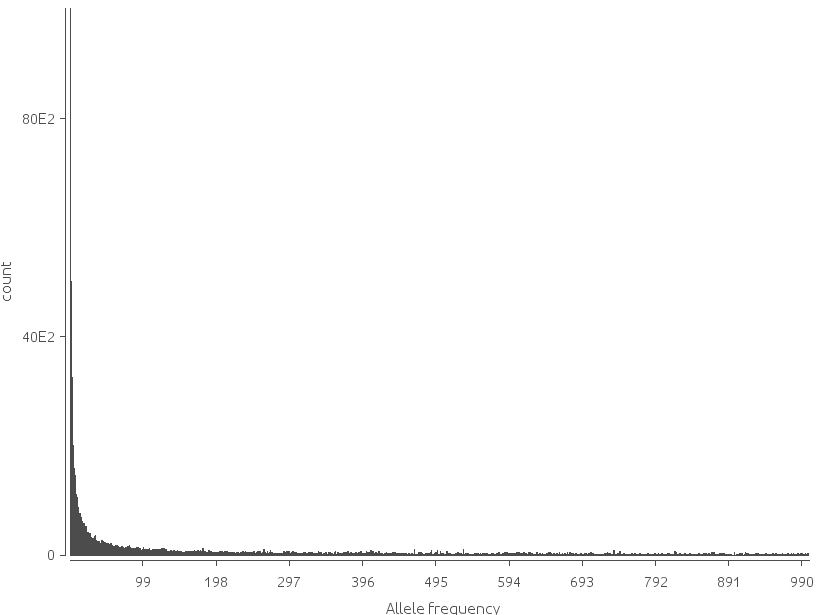
\includegraphics[width=\textwidth]{constant_size}
Tajima's D = -0.03756
\subsection{Growth at $\alpha = 100$}
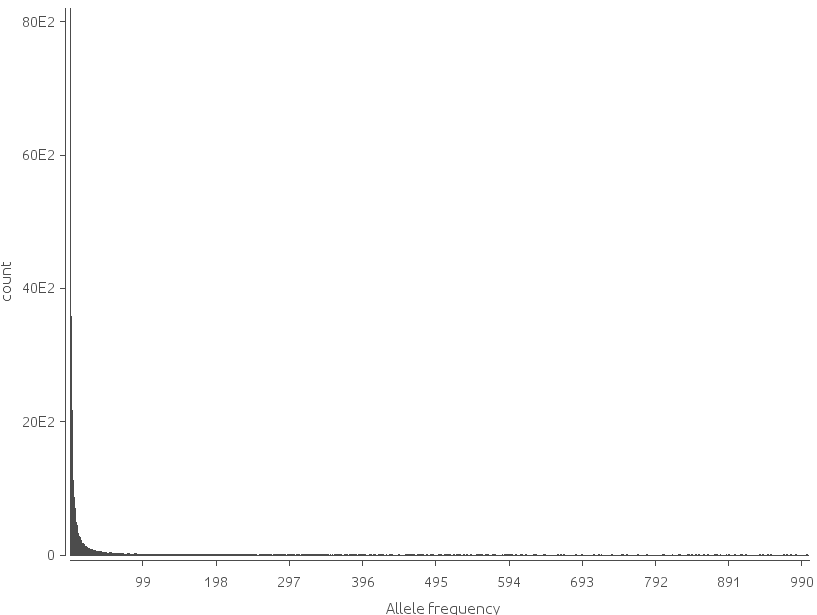
\includegraphics[width=\textwidth]{growth}
Tajima's D = -1.93785
\subsection{Bottleneck at $t=0.3$}
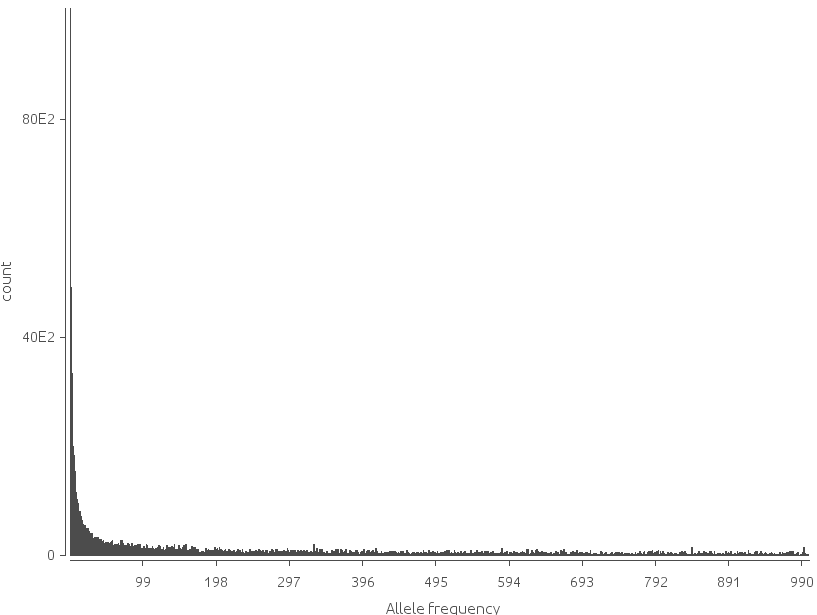
\includegraphics[width=\textwidth]{bottleneck}
Tajima's D = 0.58793

\end{document}
